\documentclass{article}
\usepackage{pgfplots}
\pgfplotsset{compat=1.16}

\begin{document}

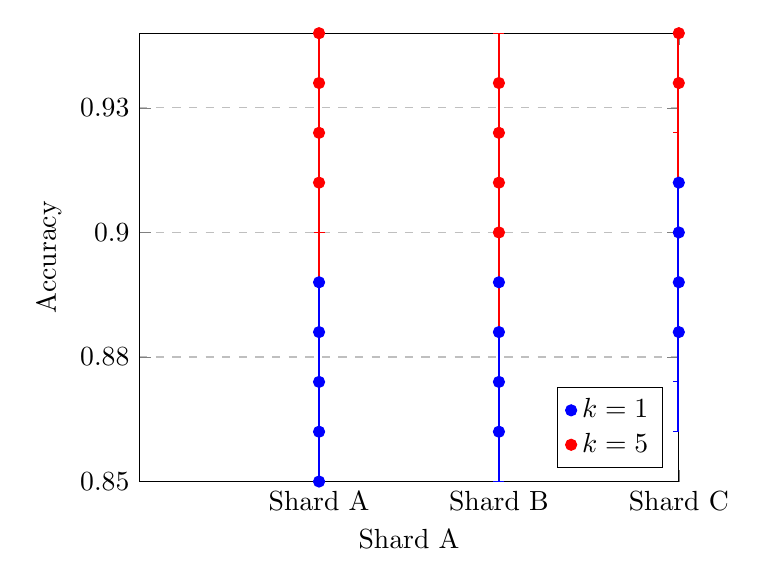
\begin{tikzpicture}
    \begin{axis}[
        xlabel={Shard A},
        ylabel={Accuracy},
        xmin=0, xmax=3,
        ymin=0.85, ymax=0.94,
        xtick={1,2,3},
        xticklabels={Shard A, Shard B, Shard C},
        ytick={0.85, 0.875, 0.9, 0.925, 0.95},
        legend pos=south east,
        ymajorgrids=true,
        grid style=dashed,
    ]
    
    % Top-1 accuracy (blue dots)
    \addplot[
        color=blue,
        mark=*,
        only marks,
        error bars/.cd,
        y dir=both,
        y explicit,
        error bar style={line width=1pt},
    ]
    coordinates {
        (1, 0.86) +-(0, 0.02)
        (1, 0.88) +-(0, 0.02)
        (1, 0.87) +-(0, 0.02)
        (1, 0.89) +-(0, 0.02)
        (1, 0.85) +-(0, 0.02)
        
        (2, 0.87) +-(0, 0.02)
        (2, 0.89) +-(0, 0.02)
        (2, 0.88) +-(0, 0.02)
        (2, 0.86) +-(0, 0.02)
        
        (3, 0.89) +-(0, 0.02)
        (3, 0.91) +-(0, 0.02)
        (3, 0.90) +-(0, 0.02)
        (3, 0.88) +-(0, 0.02)
    };
    
    % Top-5 accuracy (red dots)
    \addplot[
        color=red,
        mark=*,
        only marks,
        error bars/.cd,
        y dir=both,
        y explicit,
        error bar style={line width=1pt},
    ]
    coordinates {
        (1, 0.92) +-(0, 0.02)
        (1, 0.94) +-(0, 0.02)
        (1, 0.93) +-(0, 0.02)
        (1, 0.95) +-(0, 0.02)
        (1, 0.91) +-(0, 0.02)
        
        (2, 0.91) +-(0, 0.02)
        (2, 0.93) +-(0, 0.02)
        (2, 0.92) +-(0, 0.02)
        (2, 0.90) +-(0, 0.02)
        
        (3, 0.94) +-(0, 0.02)
        (3, 0.96) +-(0, 0.02)
        (3, 0.95) +-(0, 0.02)
        (3, 0.93) +-(0, 0.02)
    };
    
    \legend{$k=1$, $k=5$};
    
    \end{axis}
\end{tikzpicture}

\end{document}